\section{Quellencodierung}\label{sec:quellencodierung}

\subsection{Quellencodierungstheorem}\label{subsec:quellencodierungstheorem}

\begin{definition}{Codewortl\"ange}
    Sei $l_n$ die Codewortlängen.
    Die mittlere Codewortlänge $L$ einer Quelle, welche die Symbole $x_n$ mit $n = 0,\dots,N-1$ liefert, wird berechnet durch: \[L = \sum_{n=0}^{N-1} P(x_n) \cdot l_n \quad \text{[\emph{Bits/Symbol}]}\]
\end{definition}

\begin{definition}{Redundanz}
    Die Redundanz $R$ eines Codes wird berechnet durch: \[R = L - H \quad \text{[\emph{Bit/Symbol}]}\]
    Bei $R > 0$ umfasst der Code mehr Bits als nötig.
    Bei $R < 0$ reicht die Anzahl Bits pro Codewort nicht aus und Information geht verloren.
\end{definition}

\begin{definition}{Theorem zur Quellencodierung}
    Solange die Redundanz $R$ eines Codes grösser als $0$ ist, kann noch verlustfrei komprimiert werden.
    Falls $R \leq 0$, so kann nur noch verlustbehaftet komprimiert werden.
\end{definition}

\begin{subbox}{}
    \textbf{Kompressionsrate}: $R = \frac{\text{Codierte Bits}}{\text{Originale Bits}}$\\
    \textbf{Präfixfreie Codes:} Kein Code bildet den Anfang eines anderen Codes.
\end{subbox}

\subsection{Lauflängencodierung}\label{subsec:lauflangencodierung}

Die Lauflängencodierung (engl.\ Run Length Encoding, RLE) ist eine lose Sammlung von ähnlichen Methoden zur Komprimierung von Sequenzen (engl.\ Runs) identischer Symbole.
Die zentrale Idee ist, dass Ketten von identischen Zeichen zusammengefasst werden.

\textbf{Beispiel:} Die Sequenz \texttt{aaabbbcc} kann durch die Sequenz \texttt{3a3b2c} komprimiert werden.

\subsection{Huffman-Codes}\label{subsec:huffman-codes}

\begin{subbox}{Rezept Huffman-Verfahren}
    \begin{itemize}
        \item Ordne alle Symbole nach aufsteigenden Wahrscheinlichkeiten an, sie stellen die Blätter des Huffman-Baums dar.
        Gibt es Symbole mit gleicher Wahrscheinlichkeit, so spielt die Reihenfolge unter ihnen keine Rolle.
        \item Notiere unter jedem Symbol seine Wahrscheinlichkeit.
        \item Schliesse die beiden Blätter mit der kleinsten Wahrscheinlichkeit zu einem Knoten zusammen.
        Ordne dem Knoten die Summe der Wahrscheinlichkeiten der beiden Blätter zu.
        \item Wiederhole Schritt 3 so lange, bis nur noch der Stamm des Baums übrig ist.
        \item Nun wird festgelegt, ob bei jedem Knoten der linke Zweig eine 0 oder eine 1 erhält.
        Der rechte Zweig erhält dann das Komplement.
        Frei wählbar, aber muss überall einheitlich sein.
        \item Nun werden auf dem Pfad zu jedem Blatt die Nullen und Einsen ausgelesen und von links nach rechts nebeneinander geschrieben.
        Dies sind die Huffman-Codeworte.
    \end{itemize}
\end{subbox}

\subsection{LZ77}\label{subsec:lz77}

Beim LZ77-Verfahren verwenden wir Token, die aus drei Teilen aufgebaut sind: \textbf{Offset} beschreibt die Distanz zwischen dem ersten Zeichen im Vorschau und dem Ort der besten Übereinstimmung im Such-Buffer.
Die \textbf{Länge} gibt an, wie viele Zeichen übereinstimmen.
Schlussendlich wird ein \textbf{Zeichen} zusätzlich angehängt.
\begin{center}
    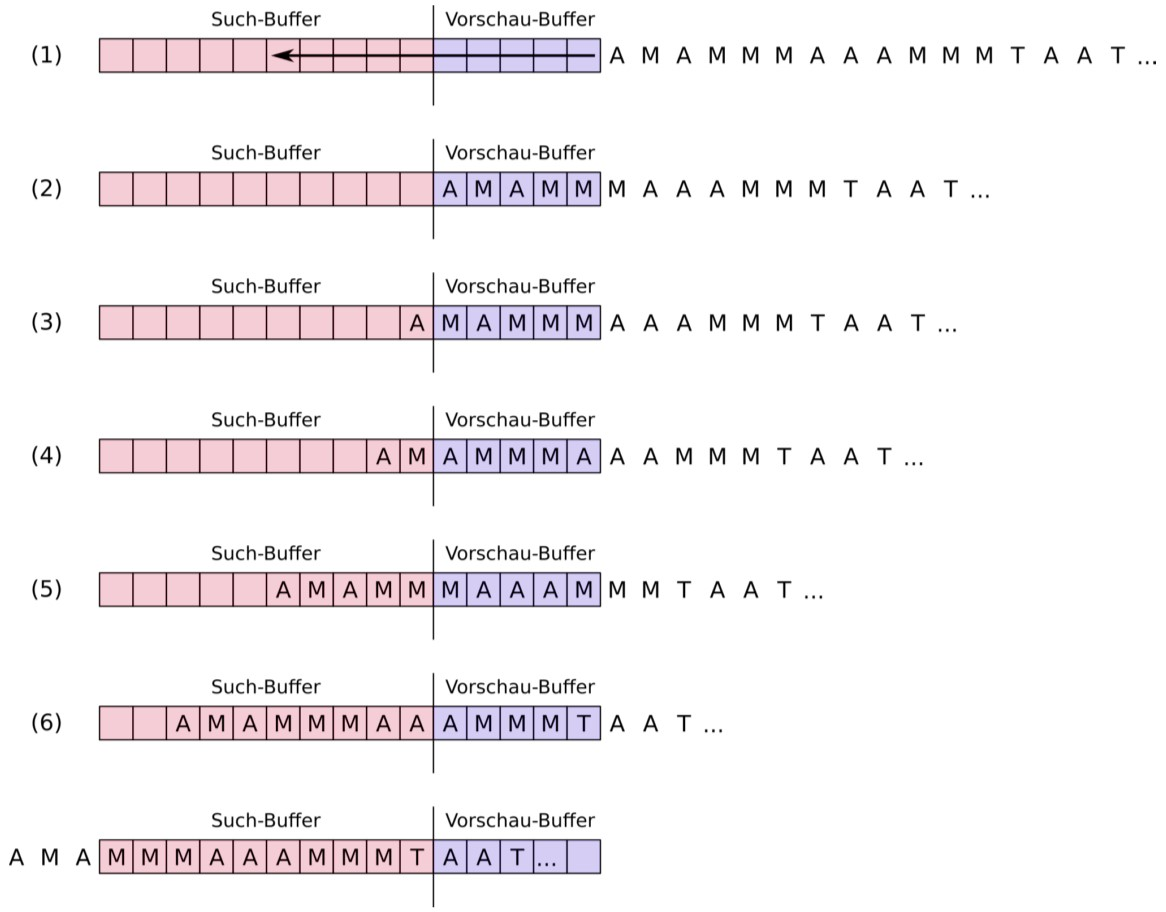
\includegraphics[scale=0.45]{LZ77-example}
\end{center}
Nach dem Ausführen des Verfahrens haben wir die Token (0,0,A), (0,0,M), (2,2,M), (4,2,A) und (6,4,T).

\subsection{LZW}\label{subsec:lzw}
\begin{center}
    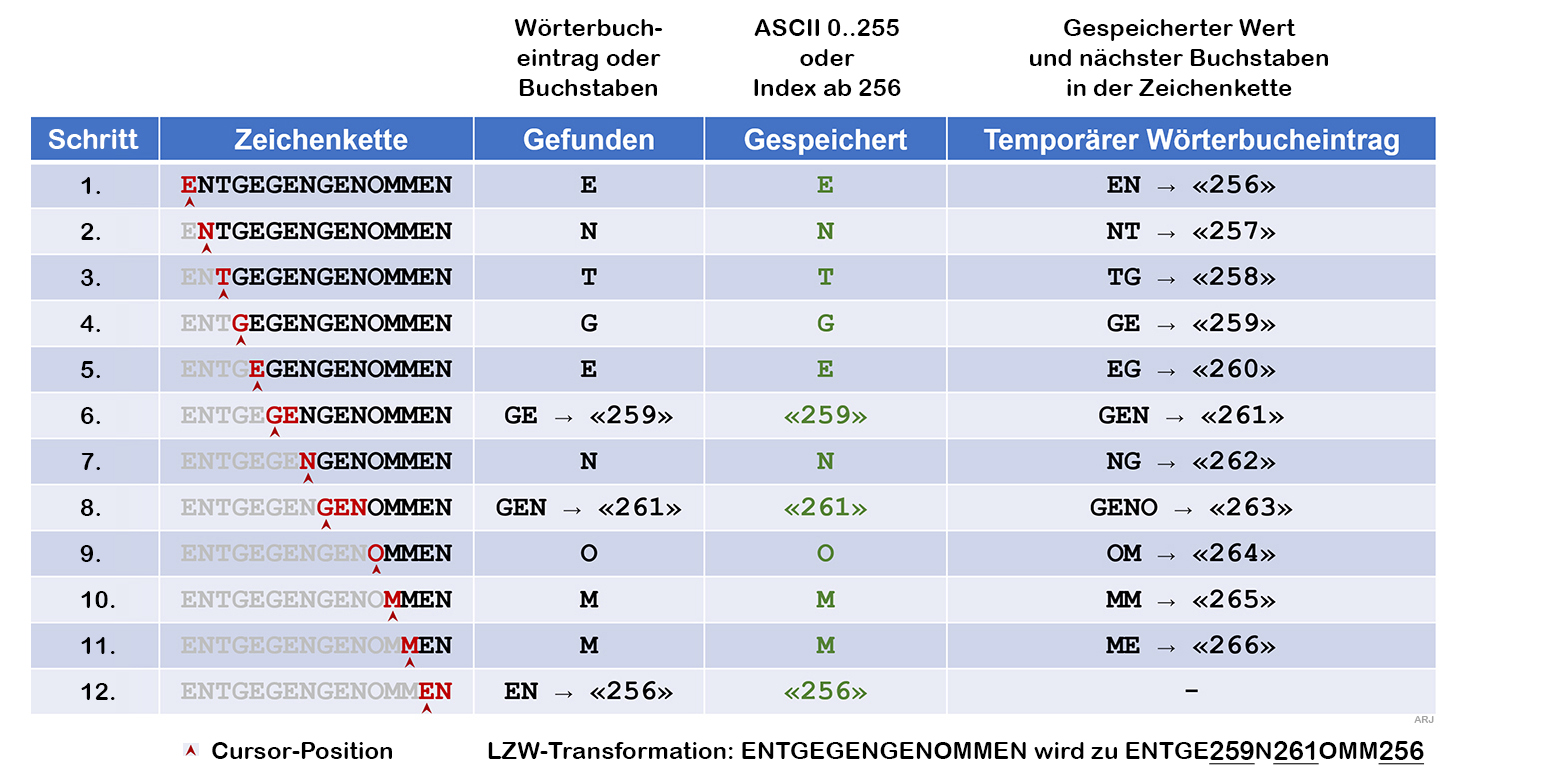
\includegraphics[scale=0.35]{LZW-example}
\end{center}